% Institute of Computer Science thesis template
% authors: Sven Laur, Liina Kamm
% last change Tõnu Tamme 09.05.2017
%--
% Compilation instructions:
% 1. Choose main language on line 55-56 (English or Estonian)
% 2. Compile 1-3 times to get refences right
% pdflatex bachelors-thesis-template
% bibtex bachelors-thesis-template
%--
% Please use references like this:
% <text> <non-breaking-space> <cite/ref-command> <punctuation>
% This is an example~\cite{example}.

\documentclass[12pt]{article}

% A package for setting layout and margins for your thesis
\usepackage[a4paper]{geometry}

% Fix long urls in footnotes
\usepackage[hyphens]{url}

\usepackage{tabularx}

%%=== A4 page setup ===
%\setlength{\paperwidth}{21.0cm}
%\setlength{\paperheight}{29.7cm}
%\setlength{\textwidth}{16cm}
%\setlength{\textheight}{25cm}


% When you write in Estonian then you want to use text with right character set
% By default LaTeX does not know what to do with õäöu letters. You have to specify
% a correct input and font encoding. For that you have to Google the Web
%
% For TexShop under MacOS X. The right lines are
%\usepackage[applemac]{inputenc}
%\usepackage[T1]{fontenc} %Absolutely critical for *hyphenation* of words with non-ASCII letters.
%
% For Windows and Linux the right magic lines are
% \usepackage[latin1]{inputenc}
% \usepackage[latin5]{inputenc}
%%\usepackage[utf8]{inputenc} %Package inputenc Error: Unicode char ´ (U+B4) not set up for use with LaTeX
\usepackage[utf8x]{inputenc}
\usepackage[T1]{fontenc} %Absolutely critical for *hyphenation* of words with non-ASCII letters.

% Typeset text in Times Roman instead of Computer Modern (EC)
\usepackage{times}

% Suggested packages:
\usepackage{microtype}  %towards typographic perfection...
\usepackage{inconsolata} %nicer font for code listings. (Use \ttfamily for lstinline bastype)


% Use package babel for English or Estonian
% If you use Estonian make sure that Estonian hyphenation is installed
% - hypen-estonian or eehyp packages
%
%===Choose the main language in thesis
%\usepackage[estonian, english]{babel} %the thesis is in English
\usepackage[english, estonian]{babel} %the thesis is in Estonian


% Change Babel document elements
\addto\captionsestonian{%
  \renewcommand{\refname}{Viidatud kirjandus}%
  \renewcommand{\appendixname}{Lisad}%
}


% If you have problems with Estonian keywords in the bibliography
%\usepackage{biblatex}
%\usepackage[backend=biber]{biblatex}
%\usepackage[style=alphabetic]{biblatex}
% plain --> \usepackage[style=numeric]{biblatex}
% abbrv --> \usepackage[style=numeric,firstinits=true]{biblatex}
% unsrt --> \usepackage[style=numeric,sorting=none]{biblatex}
% alpha --> \usepackage[style=alphabetic]{biblatex}
%\DefineBibliographyStrings{estonian}{and={ja}}
%\addbibresource{bachelor-thesis.bib}


% General packages for math in general, theorems and symbols
% Read ftp://ftp.ams.org/ams/doc/amsmath/short-math-guide.pdf for further information
\usepackage{amsmath}
\usepackage{amsthm}
\usepackage{amssymb}

% Optional calligraphic fonts
% \usepackage[mathscr]{eucal}

% Print a dot instead of colon in table or figure captions
\usepackage[labelsep=period]{caption}

% Packages for building tables and tabulars
\usepackage{array}
\usepackage{tabu}   % Wide lines in tables
\usepackage{xspace} % Non-eatable spaces in macros

% Including graphical images and setting the figure directory
\usepackage{graphicx}
\graphicspath{{figures/}}

% Packages for getting clickable links in PDF file
%\usepackage{hyperref}
\usepackage[hidelinks]{hyperref} %hide red (blue,green) boxes around links
\usepackage[all]{hypcap}


% Packages for defining colourful text together with some colours
\usepackage{color}
\usepackage{xcolor}
\definecolor{dkgreen}{rgb}{0,0.6,0}
%\definecolor{gray}{rgb}{0.5,0.5,0.5}
\definecolor{mauve}{rgb}{0.58,0,0.82}


% Standard package for drawing algorithms
% Since the thesis in article format we must define \chapter for
% the package algorithm2e (otherwise obscure errors occur)
\let\chapter\section
\usepackage[ruled, vlined, linesnumbered]{algorithm2e}

% Fix a  set of keywords which you use inside algorithms
\SetKw{True}{true}
\SetKw{False}{false}
\SetKwData{typeInt}{Int}
\SetKwData{typeRat}{Rat}
\SetKwData{Defined}{Defined}
\SetKwFunction{parseStatement}{parseStatement}


% Nice todo notes
\usepackage{todonotes}

% comments and verbatim text (code)
\usepackage{verbatim}


% Proper way to create coloured code listings
\usepackage{listings}
\lstset{
  %language=python,                % the language of the code
  language=C++,
  basicstyle=\footnotesize,        % the size of the fonts that are used for the code
  %numbers=left,                   % where to put the line-numbers
  %numberstyle=\footnotesize,      % the size of the fonts that are used for the line-numbers
  numberstyle=\tiny\color{gray},
  stepnumber=1,                    % the step between two line-numbers. If it's 1, each line
                                   % will be numbered
  numbersep=5pt,                   % how far the line-numbers are from the code
  backgroundcolor=\color{white},   % choose the background color. You must add \usepackage{color}
  showspaces=false,                % show spaces adding particular underscores
  showstringspaces=false,          % underline spaces within strings
  showtabs=false,                  % show tabs within strings adding particular underscores
  frame = lines,
  %frame=single,                   % adds a frame around the code
  rulecolor=\color{black},		   % if not set, the frame-color may be changed on line-breaks within
                                   % not-black text (e.g. commens (green here))
  tabsize=2,                       % sets default tabsize to 2 spaces
  captionpos=b,                    % sets the caption-position to bottom
  breaklines=true,                 % sets automatic line breaking
  breakatwhitespace=false,         % sets if automatic breaks should only happen at whitespace
  %title=\lstname,                 % show the filename of files included with \lstinputlisting;
                                   % also try caption instead of title
  keywordstyle=\color{blue},       % keyword style
  commentstyle=\color{dkgreen},    % comment style
  stringstyle=\color{mauve},       % string literal style
  escapeinside={\%*}{*)},          % if you want to add a comment within your code
  morekeywords={*,game, fun}       % if you want to add more keywords to the set
}

% Don't add different sized spaces to my code!
\lstset{basicstyle=\ttfamily\footnotesize,breaklines=true}


% Obscure packages to write logic formulae and program semantics
% Unless you do a bachelor thesis on program semantics or static code analysis you do not need that
% http://logicmatters.net/resources/ndexamples/proofsty3.html <= writing type rules => use semantic::inference
% ftp://tug.ctan.org/tex-archive/macros/latex/contrib/semantic/semantic.pdf
\usepackage{proof}
\usepackage{semantic}
\setlength{\inferLineSkip}{4pt}
\def\predicatebegin #1\predicateend{$\Gamma \vdash #1$}

% If you really want to draw figures in LaTeX use packages tikz or pstricks
% However, getting a corresponding illustrations is really painful


% Define your favorite macros that you use inside the thesis
% Name followed by non-removable space
\newcommand{\proveit}{ProveIt\xspace}

% Macros that make sure that the math mode is set
\newcommand{\typeF}[1] {\ensuremath{\mathsf{type_{#1}}}\xspace}
\newcommand{\opDiv}{\ensuremath{\backslash \mathsf{div}}\xspace}

% Nice Todo box
\newcommand{\TODO}{\todo[inline]}

% A way to define theorems and lemmata
\newtheorem{theorem}{Theorem}



%%% BEGIN DOCUMENT
\begin{document}

%===BEGIN TITLE PAGE
\thispagestyle{empty}
\begin{center}

\iflanguage{english}{%
\large
UNIVERSITY OF TARTU\\%[2mm]
Institute of Computer Science\\
Computer Science Curriculum\\%[2mm]
}{%
TARTU ÜLIKOOL\\
Arvutiteaduse instituut\\
Informaatika õppekava\\%[2mm]
}%\iflanguage

%\vspace*{\stretch{5}}
\vspace{25mm}

\Large Tanel Tomson

\vspace{4mm}

\huge Võrgutopoloogia visualiseerimine

%\vspace*{\stretch{7}}
\vspace{20mm}

\iflanguage{english}{%
\Large Bachelor's Thesis (9 ECTS)
}{%
\Large Bakalaureusetöö (9 EAP)
}%\iflanguage

\end{center}

\vspace{2mm}

\begin{flushright}
 {
 \setlength{\extrarowheight}{5pt}
 \begin{tabular}{r l}
  \sffamily \iflanguage{english}{Supervisor}{Juhendaja}: & \sffamily Meelis Roos, MSc \\
 \end{tabular}
 }
\end{flushright}

%\vspace*{\stretch{3}}
%\vspace{10mm}

\vfill
\centerline{Tartu 2018}

%===END TITLE PAGE

% If the thesis is printed on both sides of the page then
% the second page must be must be empty. Comment this out
% if you print only to one side of the page comment this out
%\newpage
%\thispagestyle{empty}
%\phantom{Text to fill the page}
% END OF EXTRA PAGE WITHOUT NUMBER


%===COMPULSORY INFO PAGE
\newpage

%=== Info in English
\newcommand\EngInfo{{%
\selectlanguage{english}
\noindent\textbf{\large Visualizing network topology}

\vspace*{3ex}

\noindent\textbf{Abstract:}

\noindent
The number of computers and network switches that connect the computers to a local area network can
grow large.
Maintaining an overview of the topology of those networks can get cumbersome to network
administrators.
The aim of this thesis is to write a standalone tool that is simple to use and produces a graphical
overview of the topology of a local area network for network administrators to use.

As a result a program was written.
The program asks configured network devices for information about their neighbours using the SNMP
protocool and proceeds to create a website displaying the network topology as a graph.
The installation and running of the program is simple, there is no need to install a large network
monitoring system.
Finished application was tested in the local area network of Cybernetica AS.

%Many interpreting program languages are dynamically typed, such as Visual Basic or Python. As a
%result, it is easy to write programs that crash due to mismatches of provided and expected data
%types.  One possible solution to this problem is automatic type derivation during compilation.
%In this work, we consider study how to detect type errors in the \textsc{Whitespace} language by
%using fourth order logic formulae as annotations. The main result of this thesis is a new
%triple-exponential type inference algorithm for the fourth order logic formulae. This is a
%significant advancement as the question whether there exists such an algorithm was an open
%question.
%All previous attempts to solve the problem lead lead to logical inconsistencies or required
%tedious user interaction in terms of interpretative dance. Although the resulting algorithm is
%slightly inefficient, it can be used to detect obscure programming bugs in the
%\textsc{Whitespace} language. The latter significantly improves productivity. Our practical
%experiments showed that productivity is comparable to average Java programmer.
%From a theoretical viewpoint, the result is only a small advancement in rigorous treatment of
%higher order logic formulae. The results obtained by us do not generalise to formulae with the
%fifth or higher order.

\vspace*{1ex}

\noindent\textbf{Keywords:}\\
Local area network topology, visualization, SNMP, CDP, LLDP
%Layout, formatting, template

\vspace*{1ex}

\noindent\textbf{CERCS:} P175 (Informatics, systems theory)

\vspace*{1ex}
}}%\newcommand\EngInfo


%=== Info in Estonian
\newcommand\EstInfo{{%
\selectlanguage{estonian}
\noindent\textbf{\large Võrgukommutaatorite visualiseerimine}
\vspace*{1ex}

\noindent\textbf{Lühikokkuvõte:}

%\noindent ...

Võrguadministraatori hallatavas kohtvõrgus võib arvutite ja neid kohtvõrku
ühendatavate võrgukommutaatorite arv olla suur.
Kohtvõrgu topoloogiast ülevaate saamine võib muutuda tülikaks.
Bakalaureusetöö eesmärgiks on luua lihtsasti kasutatav, eraldiseisev ja graafilist väljundit pakkuv
töövahend võrguadministraatorile kohtvõrgu topoloogiast ülevaate saamiseks.

Töö raames kirjutati programm, mis küsib seadistatud võrguseadmetelt üle SNMP protokolli andmed tema naabrite
kohta ja koostab seejärel veebilehe, kus kuvatakse seadmete topoloogia graafina.
Rakenduse paigaldamine ja käivitamine on lihtne, vajalik ei ole mahuka võrguhaldustarkvara
paigaldamine.
Valminud rakendust testiti Cybernetica AS kohtvõrgus.

\vspace*{1ex}

\noindent\textbf{Võtmesõnad:}\\
Kohtvõrgu topoloogia, visualiseerimine, SNMP, CDP, LLDP
%Layout, formatting, template

\vspace*{1ex}

\noindent\textbf{CERCS:} P175 (Informaatika, süsteemiteooria)

\vspace*{1ex}
}}%\newcommand\EstInfo


%=== Determine the order of languages on Info page
\iflanguage{english}{\EngInfo}{\EstInfo}
\iflanguage{estonian}{\EngInfo}{\EstInfo}


\newpage
\tableofcontents


% Remember to remove this from the final thesis version
% \newpage
% \listoftodos[Unsolved issues]
% \TODO{Eemalda lõplikust versioonist}
% END OF TODO PAGE


\newpage
\section{Sissejuhatus}

Võrgukommutaator (inglise keeles \textit{switch}, edaspidi ka lihtsalt kommutaator) on
võrguseade, mis ühendab seadmeid kohtvõrku.
Näiteks kontorites, kus on reeglina hulgaliselt võrguseadmeid (arvutid, printerid jne), kasutatakse
kommutaatoreid, et suur arv seadmeid saaksid kohtvõrguga ühenduda.

Võrgukommutaatoritest võib mõelda kui sorteerimisekeskustest postiteenuses.
Igal sorteerimiskeskusesse jõudval kirjal on sihtkoht, selleks on ümbrikul addressaat ja aadress.
Sorteerimiskeskuses otsustatakse, kuhu iga kiri edasi tuleb saata.
Sama ülesanne on ka võrgukommutaatoril -- otsustada, millisele ühendatud võrguseadmele iga pakett
(kiri) edasi saata.

Kommutaatoreid -- mida reeglina haldavad süsteemiadministraatorid -- võib arvutivõrgus olla mitu.
Kohtvõrgu topoloogiast (kuidas kommutaatorid üksteisega ühendatud on) ülevaate saamine võib
muutuda tülikaks ja aeganõudvaks.
Kommutaatoritelt saab küll naabrite kohta infot küsida, ent liidesed selleks on disainitud eelkõige
masinloetavaks, mis teeb nende otse kasutamise inimesele ebamugavaks.

Antud töö eesmärk on luua graafilist väljundit pakkuv eraldiseisev töövahend kohtvõrgu
topoloogiast ülevaate saamiseks.
Fookus on just kommutaatorite üksteise suhtes paiknemise visualiseerimisel, jättes
lisainformatsiooni (muud ühendatud seadmed) tagaplaanile.

Järnevalt on toodud töö struktuur.
Peatükk~\ref{sec:techintro} annab tehnilise ülevaate protokollidest, mida rakendus kasutab.
Peatükis~\ref{reqs} kirjeldatakse rakenduse jooksutamiseks vajalikud tingimused
ning enne rakenduse arendamist paika pandud nõuded.
Peatükis~\ref{similar} tuuakse ülevaade sarnast funktsionaalsust pakkuvatest
rakendustest.~\ref{usedTech} kirjeldab tehnoloogiaid ja teeke, mida programm kasutab või mida
kasutati arendusprotsessis.
Peatükis~\ref{description} tehakse detailne ja tehniline ülevaade rakenduse arhitektuurist.
Samuti põhjendatakse tehtud otsuseid ning näidatakse rakenduse nõuete täitmist ja tuuakse puudused.

\newpage
\section{Tehniline taust} \label{sec:techintro}
Järgnevalt teeme tehnilise sissejuhatuse võrguprotokollidele, mille abil saab võrguseadmetelt
haldusinfot küsida.
Antud protokollid on loodud haldusandmete jagamiseks ja loovad vundamendi meie rakenduse
kirjutamiseks.


\subsection{CDP ja LLDP}
CDP (\textit{Cisco Discovery Protocol}) ja LLDP (\textit{Link Layer Discovery Protocol}) on
mõlemad võrguprotokollid ühendatud võrguseadmetele haldusinformatsiooni jagamiseks.
LLDP ja CDP on funktsionaalsuse poolest küllaltki sarnased.
Peamine erinevus kahe protokolli vahel on, et CDP on Cisco (võrguseadmete tootja)
loodud ja hallatav omandprotokoll~\cite{cdpInfo}.
LLDP seevastu on avatud ja seadmetootjate ülene protokoll, LLDP standardit haldab
IEEE~\cite{lldpInfo}.

\subsection{SNMP} \label{subsec:snmp}
SNMP (\textit{Simple network management protocol}) on laialdaselt kasutatav
võrguhaldusprotokoll, mis kuulub OSI mudelis rakenduskihti~\cite[151]{sissejuhVorg}.
Protokoll lihtsustab ja ühtlustab võrguseadmetelt haldusinfo küsimist~\cite[151]{sissejuhVorg}.

Hallatavad seadmed hoiavad haldusinfot MIB (\textit{Management Information Base}) struktuuris,
mis on hierarhiline andmebaas~\cite[152]{sissejuhVorg}.
Igal objektil on oma unikaalne identifikaator (OID, \textit{Object Identifier})~\cite[152]{sissejuhVorg}.
Valminud rakendus kasutab konkreetseid OID-sid, et kommutaatoritelt vajalikke andmeid küsida.

SNMP protokoll defineerib päringute päises ka parameetri kogukonnasõne (\textit{community string}).
Kogukonnasõne võimaldab teha päringutele triviaalset autentimist (nt lubada andmete pärimist
vaid kindlate kogukonnasõnedega)~\cite[154-155]{sissejuhVorg}.

SNMP-st on 3 põhilist versiooni: 1, 2 ja 3~\cite[151]{sissejuhVorg}.
Valminud rakendus kasutab versiooni 2 (täpsemalt 2c).

Valminud rakendus kasutab SNMP protokolli, et võrguseadmetelt CDP ja LLDP andmeid küsida.


\newpage
\section{Rakenduse nõuded} \label{reqs}
Enne rakenduse programmeerimist pandi paika visioon sellest, kuidas ja mida rakendus tegema peab.
Vajadus oli programmi järele, mis teeks ühte konkreetset asja hästi, mitte ei prooviks
kompromissidega pakkuda suurt funktsionaalsust.
Rakenduse paigaldamine ja käivitamine peab olema lihtne, ei tohi eeldada ühegi suurema
võrguhaldustarkvara olemasolu.
Võrguadministraator peaks saama seda lihtsasti käsitsi käivitada, vastavalt enda töövoole.
Samuti peab võimalik olema programmmi automaatne perioodiline käivitamine ja tulemuse (genereeritud
veebilehe) serveerimine vabalt valitud veebiserveri kaudu.

Et kõik rakenduse eesmärkidest ühtmoodi aru saaksid, fikseeriti töö algusjärgus rakenduse nõuded,
mis järnevalt välja tuuakse.

\subsection{Kasutamise eeldused}
Rakenduse kasutamiseks on tehtud eeldus, et kasutajal on kontroll kaardistatavate võrgukommutaatorite üle.
Võrgukommutaatorid peavad olema programmi jaoks kättesaadavad ja vajalikku informatsiooni edastama.
See tähendab, et võrgukommutaatoritel peab töötama SNMP teenus ja see peab olema seadistatud jagama
CDP või LLDP andmeid.

Rakenduse jooksutamiseks on peamine riistvaraline nõue, et masinal peab olema ligipääs seadmetele,
millelt andmeid küsitakse.
Rakendus arendati peamiselt operatsioonisüsteemi Linux silmas pidades ja selle jaoks koostati ka
käivitamisjuhend ja teostati rakenduse testimine.
On tõenäoline, et rakendus toimib ka teistel operatsioonisüsteemidel, ent seda ei testitud.

\subsection{Rakenduse nõuded}
\begin{enumerate}
    \item Rakendus peab toimima vähemalt operatsioonisüsteemil Linux.
    \item Programmeerimmiskeeleks sobib Python.
    \item Rakenduse käivitamine toimub käsurealt.
    \item Võimalusel kasutame mõnda olemasolevat SNMP klienditeeki.
    \item Rakenduse sisendiks on ühe või mitme võrgukommutaatori aadress ja seadmetes seadistatud
    SNMP kommuuni nimi.
    \item \label{itm:req:diffcommunities} Kui antakse ette mitu seadet, on võimalus määrata
    erinevatele seadmetele erinevad SNMP kommuunide nimed.

    \item Rakendus küsib igalt sisendiks saadud seadmelt LLDP/CDP andmed tema enese kohtha (nimi,
    IP-aadress, ühenduste kirjeldused) ja andmed iga tema naabri kohta (nimi, IP-aadress,
    ühenduse kirjeldus).
    \item Rakendus töötleb ja vormindab saadud andmed.
    \item Tekkinud vead kuvatakse kasutajale mõistlikult (mis juhtus, mida teha).

    \item Rakendus loob antud andmete põhjal staatilise veebilehe (.html), kus kuvatakse
    graaf võrgukommutaatorite kohta.
    \item Staatilise veebilehe vaatamiseks pole vaja internetiühendust (CSS ja JS on lähtekoodiga
    kaasas, mitte ei laeta üle võrgu).
    \item Veebilehte saab vaadata ka ilma veebiserverita (üle \texttt{file://} URI-skeemi).
    \item \label{itm:req:nodesSwitches} Graafi tipud on võrgukommutaatorid.
    \item \label{itm:req:edgesSwitchConnections} Graafi servad tippude vahel on võrgukommutaatorite
    ühendused, erinevad ühenduste kiirused on tähistatud erinevalt.
    \item \label{itm:req:graphLayout}Graafis on vaikimisi paigutus mõistlik, see tähendab, et tipud
    ei kattu ja kui tekib mitu graafi, kuvatakse need üksteisest pisut eemal.
    \item \label{itm:req:dragSwitches} Graafis on võimalik seadmeid enda suva järgi lohistada.
    \item \label{itm:req:popouts} Graafis kuvatakse tippudes seadme nimi (aadress), tipule peale
    vajutades avaneb hüpikvihje.
    \item \label{itm:req:popoutsOtherDevices}Tipule peale vajutades on võimalik näha nimekirja
    kommutaatoriga ühendatud teistest seadmetest.
    \item \label{itm:req:saveChanges} Kasutaja graafile tehtud muudatused salvestatakse
    kasutaja brauseriga lokaalselt (küpsised või localstorage) ja taastatakse järgmisel avamisel.
\end{enumerate}



\newpage
\section{Sarnased lahendused} \label{similar}

Käesolevas peatüki eesmärk on tutvustada ja anda ülevaade sarnastest lahendustest,
tuues välja nende tugevused ja puudused.

\subsection{Netcrawl}
Netcrawl on lihtne programm, mille sisendiks on ühe võrguseadme aadress ja SNMP kogukonnasõne.
Rakendus küsib seejärel seadmelt naabrite info ja kordab tegevust naabrite puhul~\cite{netcrawl}.
Väljundfail on DOT-keeles\footnote{\url{https://graphviz.gitlab.io/_pages/doc/info/lang.html}}~\cite{netcrawl},
mida kasutab visualiseerimiseks Graphviz\footnote{url{https://www.graphviz.org/}} -- graafide
visualiseerimise tarkvara.
Tulemuseks on pildifail graafiga, kus on leitud võrgukommutaatorid ja nende naabrid~\cite{netcrawl}.


Netcrawl on üsna sarnane töö käigus loodava rakendusega.
Rakenduse kasutamine on lihtne ja mõne üksiku mööndusega rahuldab programm meie nõuded.
Küll aga on mõned olulised puudused.
Suurim erinevus on programmi väljundi formaat - Netcrawli kasutamisel tekib pildifail.
Nõue~\ref{itm:req:dragSwitches} täpsustab aga võimaluse kasutajal graafi tippe interaktiivselt
ümber paigutada.
Samuti paneb programm kõik leitud seadmed graafi (sh kommutaatoriga ühendatud teised seadmed) --
see tähendab, et kui seadmeid on palju, muutub graaf segaseks.
Loodud programmis tehti otsus, et kommutaatoritega ühendatud seadmeid graafis ei kuvata, vaid need
kuvatakse graafi tippudele (kommutaatoritele) vajutades
hüpikvihjetega (nõue~\ref{itm:req:popoutsOtherDevices}).
Lisaks ei saa Netcrawliga anda erinevatele kommutaatoritele erinevaid
kogukonnasõnesid (nõue~\ref{itm:req:diffcommunities}).

\subsection{Netdisco}
Netdisco on laia funktsionaalsusega võrguhaldustarkvara, mis on kirjutatud
Perlis~\cite{netdiscoDocs}.
Rakendus koosneb mitmest komponendist: taustal jooksev deemon, mis arvutivõrgu kohta andmeid pärib,
käsurealiides ja veebiserver kasutajaliidese jaoks~\cite{netdiscoDocs}.
Lisaks on rakenduse paigaldamiseks vajalik PostgreSQL andmebaas~\cite{netdiscoDocs}.

Rakendus pakub võrguseireks hulgaliselt erinevaid vaateid, sealhulgas oskab Netdisco ka seadme
naabreid kaardistada.
Selleks pakub Netdisco vaadet
\textit{Network Map}\footnote{\url{https://github.com/netdisco/netdisco/wiki/Network-Map}},
mis koostab võrguseadmetest graafi.
Antud funktsionaalsus täidab sama eesmärki, mis antud töö raames loodud rakendus.
Näiteks saab kasutaja graafis tippe ümber paigutada, asetus salvestatakse ja taastatakse lehelt
lahkudes.
Lisaks pakub Netdisco lisafunktsionaalsust, näiteks saab reaalajas kuvatavaid seadmeid filtreerida,
muuta graafi välimust ja liikuda erinevate seadmete vahel (kuvada järgmise seadme naabrid).

Peamine erinevus Netdisco ja loodud rakenduse vahel on keerukus.
Netdisco paigaldamine ja seadistamine on ajamahukam ja vajab rohkem ressursse.
Netdisco eesmärk on aidata laiemalt võrguhaldusuega, loodud rakenduse eesmärk on teha vaid üht osa.

\subsection{Switchmap}
Switchmap\footnote{\url{https://sourceforge.net/projects/switchmap/}} on tööriist
võrgukommutaatorite haldusinfo kogumiseks ja vaatamiseks.
Rakendus kogub seadmetelt üle SNMP andmed ja koostab saadud informatsiooniga veebilehe.

Erinevalt teistest kirjeldatud sarnastest rakendustest ei tee Switchmap andmete visualiseerimist,
väljund on vormistatud hoopis tabelitena.
Seetõttu sobib rakendus hästi kommutaatori ühendustest ülevaate saamiseks, aga kommutaatorite
topoloogia uurimine -- kuigi kõik selleks vajalikud andmed kuvatakse --  on visuaalse ülevaate
puudumise tõttu raskendatud.

\newpage
\section{Kasutatud tehnoloogiad} \label{usedTech}
Antud peatükis tutvustatakse prgorammeerimiskeeli, teeke ning muid vahendeid, mida valminud
rakendus kasutab.

\subsection{Keeled}
Rakenduse tagasüsteem on kirjutatud programmeerimiskeeles Python, kasutati versiooni 3.
Peamine põhjus oli, et autoril oli varasem kogemus Pythoniga juba olemas.
Samuti kontrolliti enne valiku tegemist, et leiduks sobiv SNMP teek, mis on rakenduse loomiseks
vajalik.

Kasutajaliides on loodud kasutades HTML-i ja CSS-i.
Lisaks on graafi kuvamiseks kasutatud programmeerimiskeelt Javascript.

\subsection{easySNMP} \label{easySNMP}
Kommutaatoritelt üle SNMP protokolli andmete küsimiseks kasutab rakendus Pythoni teeki easySNMP\@.
Töö algfaasis katsetati alternatiivina ka teeki PySNMP\footnote{\url{http://snmplabs.com/pysnmp}}.
Valik tehti aga easySNMP kasuks, kuna PySNMP on kommutaatoritega suhtlemisel tuntavalt aeglasem~\cite{EasySNMPDocs}.

\subsection{Cytoscape.js} \label{subsec:cyto}

Järgmiseks oli vaja Javascripti teeki graafide brauseris esitamiseks.
Andmeid visualiseerivaid (ja muuhulgas graafe toetavaid) teeke leidub arvukalt, ent autor kitsendas
otsingu lihtsuse huvides vaid graafidele spetsialiseerunud teekidele.
Samuti pidi teek olema avatud lähtekoodiga ning toetama graafi tippudele hüpikvihjete lisamist.

Kasutusele võeti Cytoscape.js\footnote{\url{http://js.cytoscape.org/}},
mis vastas kirjeldatud nõuetele~\cite{CytoscapeIntro}.
Pärast esmaseid katsetusi demodega tõusis esile hea dokumentatsioon, mis tegi teegi
kasutamise lihtsaks, lai valik erinevaid kujundusi ning graafide kuvamisel mõistlik
ekraanipinna kasutamine.

Kuigi teek vaikimisi hüpikvihjeid kuvada ei oska, on selleks loodud laiendeid.
Hüpikvihjete kuvamiseks kasutusele võetud teegid on kirjeldatud peatükis~\ref{libsUsedInUI}.

\newpage
\section{Valminud rakenduse kirjeldus} \label{description}
Rakenduse võib funktsionaalsuse järgi jagada kaheks: tagasüsteem ja kasutajaliides.
Tagasüsteemi ülesanne on küsida ja töödelda sisendiks saadud võrguseadmetelt info ühendatud
seadmete kohta.
Kasutajaliides koostab tagasüsteemi poolt saadud andmetest veebilehe kommutaatorite graafiga.
Peatükis kirjeldatakse detailselt mõlema osa arhitektuuri.

\subsection{Tagasüsteem}
Tagasüsteem on kirjutatud programmeerimiskeeles Python.
Välistest teekidest on kasutusel vaid easySNMP (\ref{easySNMP}).
Tagasüsteemi lähtekood asub \texttt{src/} kaustas (va \texttt{src/web/}, mis on kasutajaliides).

\subsubsection{Rakenduse seadistamine}
Rakenduse sätted loeb programm failist \texttt{config.ini}.
Rakenduse lähtekoodis on näidisfail \texttt{config.ini.sample}, mille rakenduse käivitaja
saab kopeerida ja vastavalt soovidele muuta.

\begin{figure} [htb]
\begin{lstlisting}[language=Python]
[Application Config]

# Default community string is used when switch has no specific community string set
defaultCommunityString = public

# Switches to be looked up.
switches = with-specific-community.example.com specificcommunity
           with-default-community.example.com
           another-with-default-community.example.com

# Enable or disable application logging (true or false)
debug = false
\end{lstlisting}
\caption{Näidis sättefail config.ini.sample}
\end{figure}

Kasutaja saab määrata kommutaatorid, millelt naabrite info küsitakse.
Seejuures saab igale kommutaatorile vajadusel määrata eraldi kogukonnasõne (vt~\ref{subsec:snmp}
ja samuti nõue~\ref{itm:req:diffcommunities}).
Lisaks on võimalik seadistada rakenduse logimist silumise tasemele (täpsemalt vt~\ref{logging}).

Rakendus kasutab sätetefaili parsimiseks Pythoni moodulit
configparser\footnote{\url{https://docs.python.org/3.6/library/configparser.html}} ja sellest
lähtuvalt on sätetefail INI-struktuuriga.
Sätetefaili puudumisel või kui sätete lugemine ebaõnnestub, kuvatakse kasutajale vastav veateade
ja programm lõpetab töö.
Sätete lugemise implementatsioon on failis \texttt{src/config\_helper.py}.

\subsubsection{Rakenduse põhivoog}

Kui sätetefailist on seadistatud kommutaatorid loetud, asutakse neilt andmeid küsima.
Seda tehakse ükshaaval, üle kommutaatorite itereerides.
Vastuseks saadud andmed hoiustab programm mälus (sõnastikuna), seejuures jagatakse iga
kommutaatori käest saadud andmed kolmeks:
\begin{enumerate}
    \item kommutaatori enda andmed (graafis tipud)
    \item kommutaatoriga ühendatud teiste kommutaatorite andmed (graafis servad)
    \item ülejäänud kommutaatoriga ühendatud seadmete info (graafi tippude hüpikvihjetes)
\end{enumerate}
Iga saadud naabri korral kontrollitakse, kas see on seadistatud kommutaator (ehk graafis teine
tipp).
Kui jah, siis talletatakse andmed, mis on vajalikud graafi serva kuvamiseks (nt portide nimed,
ühenduse kiirus).
Samas sel juhul ei kasutata naabri kohta saadud andmeid.
Teisisõnu -- eelistatakse kommutaatori andmeid, mida kommutaator ise enda kohta andis,
mitte andmeid, mida temaga ühenduses olev kommutaator tema kohta andis.
Kui naaber aga ei ole teine sisendiks saadud kommutaator (vaid kommutaatoriga ühendatud muu seade),
siis on tema kohta saadud info meile oluline ja naabri info salvestatakse.

Oluline on, et rakendus oskab kommutaatoritelt graafi koostamiseks andmeid küsida mõlema
protokolli (nii CDP kui ka LLDP) kaudu.
Kui kommutaator toetab mõlemat, siis lõpuks kuvatakse LLDP andmeid (küsitakse mõlemad,
meelde jäetakse LLDP).
Kui kommutaator kasutab vaid üht, kasutatakse seda.

\subsubsection{Päritavad andmed} \label{dataAsked}
Kommutaatorite käest küsitavad andmed võib jagada kaheks: info seadme enese kohta ja info
kommutaatoriga ühenduses olevate seadmete (naabrite) kohta.
Tabelis~\ref{tab:oids} tuuakse välja kõik andmed, mida kommutaatoritelt päritakse, sealhulgas ka SNMP
identifikaatorid (OID-d) ja MIB-struktuuride nimed (vt~\ref{subsec:snmp}).

Seadmetelt andmete küsimiseks kasutatakse easySNMP (vt~\ref{easySNMP}) teegi funktsiooni
session.walk()\footnote{\url{https://easysnmp.readthedocs.io/en/latest/session\_api.html}}.
Funktsioon teeb sisemiselt SNMP GetNextRequest päringu.

\begin{table}[p]
\small
\centering
\caption{Muutujad, mis üle SNMP küsitakse}
    \begin{tabular}{| p{4cm} | p{3.2cm} | p{1.2cm} | p{4.3cm} |}
    \hline
        OID & Muutuja nimi & MIB & Kirjeldus \\
    \hline
        1.3.6.1.4.1.9.9.23.1.3.4.0 & cdpGlobalDeviceId & CISCO-CDP-MIB & Seadme id (nimi). Kasutatakse sisemiselt unikaalse identifikaatorina teiste CDP päringute jaoks \\
    \hline
        1.3.6.1.4.1.9.9.23.1.2.1.1.6 & cdpCacheDeviceId & CISCO-CDP-MIB & Ühendatud seadme nimi \\
    \hline
        1.3.6.1.4.1.9.9.23.1.2.1.1.4 & cdpCacheAddress & CISCO-CDP-MIB & Ühendatud seadme IP-aadress \\
    \hline
        1.3.6.1.4.1.9.9.23.1.2.1.1.7 & cdpCacheDevicePort & CISCO-CDP-MIB & Ühendatud seadme pordi kirjeldus (ühendatud seadme poolel) \\
    \hline
        1.3.6.1.2.1.2.2.1.2 & ifDesc & IF-MIB & Ühenduse kirjeldus (kommutaatori poolel) \\
    \hline
        1.0.8802.1.1.2.1.3.3.0 & lldpLocSysName & LLDP-MIB & Seadme nimi. Kasutatakse sisemiselt unikaalse identifikaatorina teiste LLDP päringute jaoks \\
    \hline
        1.0.8802.1.1.2.1.3.7.1.3 & lldpLocPortId & LLDP-MIB & Ühendatud pordi kirjeldus (kommutaatori poolel) \\
    \hline
        1.0.8802.1.1.2.1.4.1.1.9 & lldpRemSysName & LLDP-MIB & Ühendatud seadme nimi \\
    \hline
        1.0.8802.1.1.2.1.4.1.1.7 & lldpRemPortId & LLDP-MIB & Ühendatud pordi id (ühendatud seadme poolel) \\
    \hline
        1.0.8802.1.1.2.1.4.1.1.8 & lldpRemPortDesc & LLDP-MIB & Ühendatud pordi kirjeldus (ühendatud seadme poolel) \\
    \hline
        1.0.8802.1.1.2.1.4.2.1.4 & lldpRemManAddrIfId & LLDP-MIB & Ühendatud seadme IP-aadress \\
    \hline
\end{tabular}
\label{tab:oids}
\end{table}

\subsubsection{Andmete faili salvestamine} \label{backendOutput}
Et andmed jõuaksid tagasüsteemilt kasutajaliidesesse, kirjutatakse need Javascripti lähtekoodi
faili.
Põhjus, miks kasutatakse Javascripti faili (laiendiga \texttt{.js}) ja mitte näiteks JSON-formaati,
on kirjeldatud peatükis~\ref{dataInput}.
Andmed itereeritakse ja vormindatakse vastavalt~\nameref{subsec:cyto} teegi sisendformaadile.
Andmete faili kirjutamise implementatsioon on failis \texttt{src/output\_helper.py}.

\subsubsection{Veahaldus}
Vigadele kõige altim on kommutaatoritelt andmete küsimine -- juhul kui kommutaatoriga ei saada
ühendust (vale seadistus, võrguprobleem vms).
Veahalduse roll on sel juhul tagada, et programmi töö jätkuks teistelt kommutaatoritelt andmete
küsimisega.
Sel juhul logitakse kasutajale olemasolevate andmetega võimalikult informatiivne viga ja minnakse
programmi vooga edasi.

\subsubsection{Logimine} \label{logging}
Logimiseks kasutatakse Pythoni moodulit
logging\footnote{\url{https://docs.python.org/3.6/library/logging.html}}.
Rakenduse sättefailis on võimalik määrata logimise taset (\texttt{debug},
kui \texttt{debug = true} või \texttt{info}, kui \texttt{debug = false}).
\texttt{Debug} tasemel logikirjed on mõeldud vaid arendamiseks ja vigade silumiseks.


\subsection{Kasutajaliides}
Kasutajaliides on staatiline veebileht.
Kasutajaliidese töö on kuvada tagasüsteemi poolt loodud andmed graafina kasutaja brauseris.
Kasutajaliidese lähtekood asub \texttt{src/web/} kataloogis.

\subsubsection{Välised teegid} \label{libsUsedInUI}
Graafide kuvamiseks kasutatakse Javascripti teeki cytoscape.js (\ref{subsec:cyto}).
Lisaks kasutatakse laiendit
cytoscape-popper\footnote{\url{https://github.com/cytoscape/cytoscape.js-popper}}, mis lisab
cytoscape.js-le Popper.js\footnote{\url{https://popper.js.org}} (teek muuhulgas hüpikvihjete
kuvamiseks) toe.
Lisaks võeti kasutusele Tippy.js\footnote{\url{https://atomiks.github.io/tippyjs/}},
mis teeb hüpikvihjete loomise ja kohandamise Popper.js-iga lihtsamaks.

Välised teegid asuvad kataloogis \texttt{src/web/lib/}.
Kõik kasutatud välised failid on lähtekoodiga kaasas (ei laeta internetist).
Põhjuseks turvalisus ja võimalus rakendust ilma võrguühenduseta kasutada.

\subsubsection{Lokaalse faili laadimine brauseris}
Lokaalsel veebilehel lokaalse faili Javascriptiga lugemine on keerulisem kui võiks arvata.
Brauserid kaitsevad kasutajaid pahatahtliku koodi laadimise ja jooksutamise eest, aga samamoodi
piiratakse ka pääsu kasutaja lokaalsetele failidele.

Brauserid rakendavad reeglina doomenisisese ressursikasutuse (\textit{same-origin policy})
printsiipi.
See tähendab, et veebileht ei saa jooksutada koodi ning ei pääse ligi failidele, mis asuvad
teistes domeenides.
Et võimaldada ka doomenivälist ressursikaasutust on W3C loonud spetsifikatsiooni CORS
(\textit{Cross-origin resource sharing})~\cite{W3CORS}.


Antud spetsifikatsiooni implementeerivad brauserid ise ning sellele on erinevad arendajad
lähenenud erinevalt~\cite{localWebSec}.
Loodud programmi kontekstis tuli esile probleem, et kasutades \texttt{file://} URI-skeemi, on faili
päritolu (\textit{origin}) definitsioon CORS-i spetsifikatsioonis
lahtine~\cite[peatükk 4, punkt 4]{ietfOrigin}.
See tähendab, et brauserid käituvad antud olukorras erinevalt ja ei ole garantiid, et igas
brauseris tagasüsteemi poolt loodud faili lugemine õnnestub.
Chromium (ja Google Chrome) ei lubanud veebilehel \texttt{file://} URI-skeemiga lokaalset faili
üldse laadida.
Firefox lubaks faili laadida, aga (alates küljendusmootori Gecko versioonist 1.9) seab ette nõuded
faili asukohale~\cite{FFCORS}.

\subsubsection{Tagasüsteemi loodud sisendi lugemine} \label{dataInput}
Töö autor lootis algselt kommutaatorite andmed tagasüsteemilt kasutajaliidesele edastada
JSON-formaadis, seejuures kasutada Pythoni ja Javascripti standardteeke.
Katsetuste käigus tuli aga välja eelnevalt kirjeldatud brauserite erinev käitumine.

Kasutaja brauserite kohta eeldusi teha ei tahetud -- programm peaks töötama sõltumata brauserist.
Üks lahendus oleks veebirakenduse kuvamiseks kasutada lokaalset veebiserverit ja küsida andmefail
üle \texttt{http://} URI-skeemi
\footnote{\url{https://stackoverflow.com/questions/46258449/cors-error-requests-are-only-supported-for-protocol-schemes-http-etc}}
\footnote{\url{https://stackoverflow.com/questions/20041656/xmlhttprequest-cannot-load-file-cross-origin-requests-are-only-supported-for-ht}}
\footnote{\url{https://stackoverflow.com/questions/35335047/how-to-get-rid-of-cross-origin-request-block-in-chrome}}.
See on aga töö raames loodava rakenduse kontekstis üleliigne keerukus ja probleemi lahenduseks ei
sobinud.

Selle asemel otsustati andmed tagasüsteemi poolt vormindada Javascripti koodifailiks.
Fail defineerib ühe muutuja, milles on kommutaatorite andmed sõnastikus.
Seejuures vormindatakse andmed sõnastikus nõnda, et selle saab otse cytoscape.js
(vt~\ref{subsec:cyto}) teegile ette anda.
See tähendab, et sõnastikus on elemendid \texttt{nodes} ja \texttt{edges}, vastavalt graafi tipud
ja servad.
Antud fail laetakse kasutajaliideses Javascripti lähtekoodina ja seejärel on kommutaatorite
andmed kasutajaliideses olemas ja neid saab kasutajale kuvada.

\subsubsection{Graafi kuvamine} \label{graphDisplay}
Kuna sisendandmed on juba tagasüsteemi poolt teegile cytoscape.js loetavaks vormindatud, on
graafi kuvamiseks vajalik vaid cytoscape.js seadistada.
Peamine otsus, mis tuli teha, oli küljenduse
valimine\footnote{\url{http://js.cytoscape.org/\#layouts}}.
Hea küljendus kasutab kogu ekraanipinna ära (jaotab tipud laiali) ja samuti asetab tipud nõnda, et
servad ei kattuks (vt nõue~\ref{itm:req:graphLayout}).
Autori katsetustest tuli välja, et küljendus \texttt{breadthfirst} kasutas ekraanipinda kõige
mõistlikumalt -- see võeti ka kasutusele.
Välja tasub tuua ka \texttt{concentric} küljendus, mis toimis samuti hästi, ent mitme graafi
kuvamisel jäi viimane hätta kogu ekraanipinna ära kasutamisega.

Graafi kujunduses võeti aluseks cytoscape.js-i demo
\textit{linkout-example}~\footnote{\url{http://js.cytoscape.org/demos/linkout-example}}.
Samas lisati tippudes tekstile kontrasti (must taust), et lugemist lihtsustada.
Graafi kuvamine on implementeeritud failis \texttt{src/web/code.js}.

Graafi tippudeks on kommutaatorid, millelt andmeid küsiti (nõue~\ref{itm:req:nodesSwitches}).
Servadeks on ühendused kommutaatorite vahel (nõue~\ref{itm:req:edgesSwitchConnections}).
Seejuures kuvatakse servadel ka mõlema kommutaatori port, mille kaudu nad ühendatud on.
Algselt oli plaanis servadel kuvada ühenduste kiirused, kuid otsustati pordi nimede kasuks, sest
nimi sisaldab lisaks pordi numbrile infot ka kiiruse kohta (Gi on 1000Mbps, Fa on 100Mbps jne).

Joonisel~\ref{fig:graph} on toodud kuvatõmmis programmi poolt loodud graafist.

\begin{figure} [ht] %try to place the figure here (next option top of the page)
\begin{center}
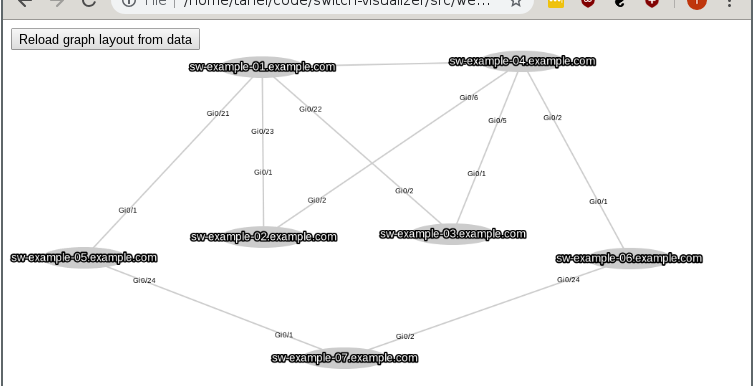
\includegraphics[width=1\textwidth]{graph}
    \caption{Näidis rakenduse poolt loodud graafist (nimed muudetud).}
\label{fig:graph}
\end{center}
\end{figure}

\subsubsection{Hüpikvihjed}
Vastavalt nõuetele~\ref{itm:req:popouts} ja ~\ref{itm:req:popoutsOtherDevices}, peavad tippudele
vajutades avanema hüpikvihjed.
Nagu peatükis~\ref{libsUsedInUI} juba kirjeldati, implementeeriti hüpikvihjed teegiga Tippy.js, mis
sisemiselt kasutab Popper.js teeki.
Popper.js teegi cytoscape.js teegiga integreerimiseks kasutati cytoscape-popper laiendit.

Autori roll hüpikvihjete tööle saamiseks oli Tippy.js implementatsioon seadistada.
Tippy pakub mitmeid kujundusi\footnote{\url{https://atomiks.github.io/tippyjs/themes}}.
Autor valis läbipaistva kujunduse, et hüpikaknad ei kataks ära hüpikakna all olevaid graafi
servasid.
Hüpikvihjete avamine ja sulgemine (mõlemad tipule vajutades) implementeeeriti Tippy.js teegi
väliselt eraldi, eesmärgiga, et korraga oleks võimalik avada mitu vihjet.

Vihjete sisu koostatakse Javascriptiga, andmed saadakse samast tagasüsteemi poolt loodud
sisendfailist, mille põhjal ka graaf tehakse.
Hüpikvihjes kuvatakse kõik kommutaatoriga ühendatud seadmed, välja arvatud sätetes määratud
kommutaatorid.
Hüpikvihjete implementatsioon on samuti failis \texttt{src/web/code.js}.

Joonisel~\ref{fig:tooltip} on toodud kuvatõmmis programmi poolt loodud graafist.

\begin{figure} [ht] %try to place the figure here (next option top of the page)
\begin{center}
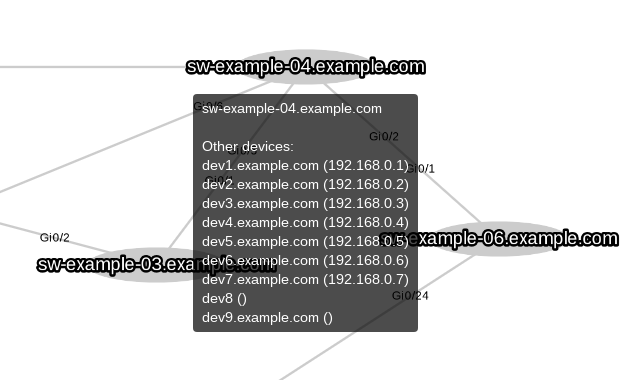
\includegraphics[width=1\textwidth]{tooltip}
    \caption{Näidis graafi hüpikvihjest (nimed ja IP-aadressid muudetud).}
\label{fig:tooltip}
\end{center}
\end{figure}

\subsubsection{Kasutaja muudatuste salvestamine} \label{saveChanges}
Vastavalt nõudele~\ref{itm:req:saveChanges} pidi kasutajaliides salvestama kasutaja muudatused
graafile (tippude asukohtade muudatused).
Antud funktsionaalsust teek cytoscape.js otse ei paku, küll aga defineeritakse funktsioon
\texttt{cy.json()}\footnote{\url{http://js.cytoscape.org/\#cy.json}}, mis võimaldab graafi paigutust
JSON-formaadis importida ja eksportida.

Implementeeriti graafi asetuse salvestamine, kui kasutaja veebilehelt lahkub või seda värskendab.
JSON andmed salvestatakse sõnena brauseri lokaalsesse andmesalvestisse
(localStorage\footnote{\url{https://developer.mozilla.org/en-US/docs/Web/API/Window/localStorage}}).
Kui kasutaja veebilehe avab, laetakse ja taastatakse graafi paigutus andmesalvestist.
Kui seda varasemalt salvestatud ei ole (esimene külastus), siis laetakse graaf andmefailist.
Brauseri lokaalne andmesalvesti on domeenipõhine, seega kui antud rakendut on erinevate domeenide
taga, siis need üksteist ei sega.
Samuti lisati veebilehele nupp graafi paigutuse taastamiseks -- graafi andmefailist uuesti
laadimiseks.

\subsection{Lähtekood ja litsents}
Rakenduse lähtekood on üleval Github keskkonnas: \url{https://github.com/taneltomson/switch-visualizer}.
Autor valis lähtekoodile MIT-litsentsi.

\subsection{Rakenduse puudused}
Järnevalt toob töö autor valminud rakenduse puudused ja võimalikud edasiarendused.

\subsubsection{Tekst graafi servadel}
Nagu peatükis~\ref{graphDisplay} mainiti, kuvatakse graafi servadel mõlema seadme (tipu) lähedal
lipikud ühenduse pordi infoga.
Seda tehakse teegi cytoscape.js poolt pakutava
funktsionaalsusega Lipikud\footnote{\url{http://js.cytoscape.org/\#style/labels}}.
Teek võimaldab määrata nihke (kauguse tipust), kus lipikut kuvada.
Töö autor määras selleks kauguseks 90 pikslit.

Üldjuhul töötavad lipikud nagu eeldada võiks -- lipik, mis on tipule lähemal, kirjeldab just selle
tipu ühendust.
Probleem ilmneb, kui programmi kasutaja veab tipud üksteisele väga lähedale.
Kuna lipiku kaugus tipust on fikseeritud (90 pikslit), siis kui tipud on üksteisele lähemal kui ca
180 pikslit,
vahetavad lipikud kohad ja jääb mulje, et lipikud lähevad vahetusse (annavad infot teise tipu
kohta).

Töö autor proovis probleemi leevendamiseks tuua lipikud tippudele lähemale.
Siis tekib aga probleem, et lipikud võivad jääda tipu alla, sest tipus kuvatakse seadme nimi (tipp
on ristkülikukujuline, horisontaalselt lai).
Lõpuks kasutusele võetud 90 pikslit oli kompromiss, mis tehtud katsetuste puhul kõige paremini töötas.

\subsubsection{Andmete uuenemise märkamine}
Rakenduse kasutajaliides salvestab muudatused, mida kasutaja graafile teeb (vt~\ref{saveChanges}).
Tegelikult tähendab see ka seda, et salvestatakse tagasüsteemi poolt küsitud andmed ja need
laetakse järgmisel külastusel.
Seega on võimalik olukord, kus taustal on tagasüsteem kommutaatoritelt uued andmed küsinud, aga
kasutajaliides kuvab veel vanu andmeid.

Ideaalne lahendus oleks siin see, kui programm oskaks teha tagasüsteemi poolt loodud andmetele
sisulist võrdlust.
See tähendab, et saaks aru, kui on toimunud sisuline muutus, kus näiteks mõni seade on lisandunud
või eemaldatud.
Seejuures ignoreerides mittesisulisi muutusi, näiteks kui mõne seadme järjekord loetelus on
vahetunud.

Veidi lihtsam lahendus oleks, kui kasutajaliides salvestaks koos kasutaja muudatustega ka
andmefailist (mille põhjal graaf loodi) arvutatud räsi.
Antud räsi saaks igal veebilehe avamisel (kui laetakse kasutaja poolt muudetud graaf) võrrelda
andmefaili räsiga ning kui need on muutunud, kasutajale teade kuvada.

\subsubsection{Ilma veebiserverita mitme rakenduse instanssi kasutamine}
Andmete brauseri lokaalsesse andmesalvestisse salvestamisega on ka teine probleem.
Nagu peatükis \ref{saveChanges} juba mainiti, on brauseri andmesalvesti domeenipõhine.

Samas vähemalt Chromium arvestab kõik failid, mis on avatud üle \texttt{file://} URI-skeemi ühte
domeeni kuuluvaks.
See tähendab, et ilma veebiserverita saab korraga kasutada vaid üht rakenduse instanssi, või
täpsemalt vaadata vaid üht tagasüsteemi poolt loodud graafi korraga.

Probleemi saaks lahendada, kui lisada (juhul, kui kasutajaliidest vaadatakse üle \texttt{file://}
URI-skeemi) ka märge faili asukoha kohta ja kasutajaliidese avamisel kontrollida, et varasemalt
salvestatud andmed on salvestatud sama rakenduse instanssi poolt.

\clearpage
\section{Kokkuvõte}

Antud bakalaureusetöö raames kirjutas autor rakenduse, mis abistab võrgutopoloogia
visualiseerimisel.
Rakendus on ennekõike mõeldud võrguadministraatoritele oma kontrolli all olevate seadmete (peamiselt
võrgukommutaatorite) topoloogia vaatamimseks ja probleemide avastamiseks.
Selleks küsib rakendus sisendiks antud seadmetelt üle SNMP andmed seadme enese ja tema naabrite
kohta, töötleb vastused ja koostab tulemustest veebilehe graafiga.

Kuigi rakendus loodi vaid kommutaatorite topoloogiat silmas pidades, ei pea programmi kasutamisel
piirduma rangelt 2. kihi kohtvõrguga.
Ka ruuterid ja tulemüürid oskavad üle SNMP andmeid jagada, nii et teoreetiliselt on võimalik
programmiga luua graafe ka üle mitme kohtvõrgu.

Rakendust testiti Cybernetica AS kohtvõrgus.
Arenduse käigus kasutas töö autor programmi testimiseks piiratud arvu võrguseadmeid.
Arendusprotsessi lõpus testis programmi ka võrguadministraator suurema hulga võrguseadmetega ja
rakendus täitis seatud eesmärgi.

Rakenduse edasiseks täiendamiseks on mitmeid võimalusi.
Kasutusmugavus paraneks, kui rakendus saaks ise aru, kui taustal on andmed muutunud (seadmete
topoloogia muutus võrreldes viimase seisuga) ja annaks sellest kasuatajaliideses märku.
Samuti saaks lisada rohkem andmeid, mida programm seadmete kohta küsib ja kuvab.









%
%
%\newpage
%\subsection{Title of Subsection 2}
%
%Rule: If you divide the text into subsections (or subsubsections) then there has to be at least two of them, otherwise do not create any.
%
%Tip: You can also use paragraphs, e.g.
%\paragraph{Type rules for integers.} Some text ...
%
%\paragraph{Type rules for rational numbers.} Some text here too...
%
%
%
%
%\subsection{How to use references} \label{sec:using_ref}
%
%\paragraph{Cross-references to figures, tables and other document elements.}
%LaTeX  internally numbers all kind of objects that have sequence numbers:
%\begin{itemize}
%\item chapters, sections, subsections;
%\item figures, tables, algorithms;
%\item equations, equation arrays.
%\end{itemize}
%To reference them automatically, you have to generate a label using \texttt{$\backslash$label\{some-name\}} just after the object that has the number inside. Usually, labels of different objects are split into different namespaces by adding dedicated prefix, such as \texttt{sec:}, \texttt{fig:}. To use the corresponding reference, you must use command \texttt{$\backslash$ref} or \texttt{$\backslash$eqref}. For instance, we can reference this subsection by calling Section~\ref{sec:using_ref}. Note that there should be a nonbreakable space \texttt{\~} between the name of the object and the reference so that they would not appear on different lines (does not work in Estonian).
%
%
%
%\paragraph{Citations.}
%Usually, you also want to reference articles, webpages, tools or programs or books. For that you should use citations and references. The system is similar to the cross-referencing system in LaTeX. For each reference you must assign a unique label. Again, there are many naming schemes for labels. However, as you have a short document anything works. To reference to a particular source you must use \texttt{$\backslash$cite\{label\}} or \texttt{$\backslash$cite[page]\{label\}}.
%
%References themselves can be part of a LaTeX source file. For that you need to define a bibliography section. However, this approach is really uncommon. It is much more easier to use BibTeX to synthesise the right reference form for you. For that you must use two commands in the LaTeX source
%\begin{itemize}
%\item $\backslash$bibliographystyle\{alpha\} or $\backslash$bibliographystyle\{plain\}
%\item $\backslash$bibliography\{file-name\}
%\end{itemize}
%The first command determines whether the references are numbered by letter-number combinations or by cryptic numbers. It is more common to use \texttt{alpha} style. The second command determines the file containing the bibliographic entries. The file should end with \texttt{bib} extension. Each reference there is in specific form. The simplest way to avoid all technicalities is to use graphical frontend  Jabref (\url{http://jabref.sourceforge.net/}) to manage references. Another alternative is to use DBLP database of references and copy BibTeX entries directly form there.
%
%
%The following paragraph shows how references can be used. Game-based proving is a way to analyse security of a cryptographic protocol~\cite{GameB_1, GameB_2}. There are automatic provers, such as {CertiCrypt\-}~\cite{certicrypt} and ProVerif~\cite{proVerif}.
%
%
%
%\newpage
%\section{How to add figures and pictures to your thesis}
%
%
%Here are a few examples of how to add figures or pictures to your thesis (see Figures~\ref{fig:fnCompModel}, \ref{fig:game-based_proofs}, \ref{fig:proveit_screenshot}).
%
%Rule: All the figures, tables and extras in the thesis have to be referred to somewhere in the text.
%
%
%\begin{figure} [ht] %try to place the figure here (next option top of the page)
%\begin{center}
%\includegraphics[width=0.8\textwidth]{computational_model_function}
%\caption{The title of the Figure.}
%\label{fig:fnCompModel}
%\end{center}
%\end{figure}
%
%
%
%\begin{figure} [!ht] %if [h] doesn't work, we can force with !
%\begin{center}
%\includegraphics[width=\textwidth]{game-based_proofs}
%\caption{Refer if the figure is not yours~\cite{kamm12}.}
%\label{fig:game-based_proofs}
%\end{center}
%\end{figure}
%
%
%\begin{figure} [p]
%\begin{center}
%\includegraphics[width=\textwidth]{proveit_screenshot}
%\caption{Screenshot of \proveit.}
%\label{fig:proveit_screenshot}
%\end{center}
%\end{figure}
%
%Tip: If you add a screenshot then labeling the parts might help make the text more understandable (panel C vs bottom left part), e.g.
%
%
%\begin{figure} [htbp]
%\begin{tabular}{c c}
%%
%\begin{minipage}{0.45\textwidth}
%\includegraphics[width=\textwidth]{LCA_2_solutions}
%\end{minipage}
%%
%&
%\begin{minipage}{0.55\textwidth}
%\centering
%\begin{tabular}{ l | l |}
%	Node & Decendants \\ \hline
%  1 & 2, 3, 4 \\ \hline
%  2 & 3, 4 \\ \hline
%  3 & \\ \hline
%  4 & \\ \hline
%  5 & 3, 4, 6, 7 \\ \hline
%  6 & 4 \\ \hline
%  7 & 3 \\  \hline
%  8 & 3, 4, 5, 6, 7\\ \hline
%  9 & 3, 4, 5, 6, 7\\ \hline
%\end{tabular}
%\end{minipage}
%\end{tabular}
%%
%\caption{Example how to put two figures parallel to each other.}
%\label{fig:LCA_2_solutions}
%\end{figure}
%
%
%Example: A screenshot of \proveit can be seen on Figure~\ref{fig:proveit_screenshot}. The user first enters the pseudocode of the initial game in panel B. \proveit also keeps track of all the previous games showing the progress on a graph seen in panel A.
%
%There are two figures side by side on Figure~\ref{fig:LCA_2_solutions}.
%
%
%
%\clearpage %if newpage doesn't work
%\section{Other Ways to Represent Data}
%
%\subsection{Tables}
%
%\begin{table}[h]
%\centering
%\caption{Statements in the \proveit language.}
%\begin{tabular}{| l | l |}
%	\hline
%	\bf{Statement} & \bf{Typeset Example} \\
%	\hline
%	assignment & $a := 5 + b$ \\
%	\hline
%	uniform choice & $m <- M$ \\
%	\hline
%	function signature & $f : K \times M -> L$\\
%	\hline
%\end{tabular}
%\label{tab:statements}
%\end{table}
%
%
%\subsection{Lists}
%
%Numbered list example:
%\begin{enumerate}
%	\item item one;
%	\item item two;
%	\item item three.
%\end{enumerate}
%
%\subsection{Math mode}
%Example:
%\begin{equation}
%a + b = c + d
%\end{equation}
%Aligning:
%\begin{align*}
%	a &= 5 \\
%	b + c &= a \\
%	a -2*3 &= 5/4
%\end{align*}
%Hint: Variables or equations in text are separated with \$ sign, e.g. $a$, $x - y$.
%
%\paragraph{Inference Rules}
%\[
%	\inference[addition]{x : T & y : T}{x + y : T}
%\]
%Bigger example:
%\[
%\inference[assign]{c := a + b &
%	\inference[addG]{a : \typeRat &
%		\inference[var]{b : \typeInt & \typeInt \subseteq \typeRat}{b : \typeRat}
%		}{a + b : \typeRat}
%	}{c : \typeRat}
%\]
%
%
%\subsection{algorithm2e}
%
%\begin{algorithm} [!h]
%	\caption{typeChecking} \label{alg:typeChecking}
%	\KwIn{Abstract syntax tree}
%	\KwResult{Type checking result; In addition, type table \typeF{type\_G} for global variables, \typeF{game} for the main game and \typeF{fun} for each $fun \in F$}
%	\SetKwData{s}{s}
%	\BlankLine
%
%	\While{something changed in last cycle}{
%		\lForEach{global statement \s} {
%			\parseStatement{\s, \typeF{type\_G}}\;
%		}
%		\ForEach{function $fun$} {
%		\lForEach{statement \s in $fun$} {
%			\parseStatement{\s, \typeF{fun}}\;
%		}
%		}
%		\lForEach{statement \s in game} {
%			\parseStatement{\s, \typeF{game}}\;
%		}
%	}
%	%\eIf{error messages were found}{\Return \False\;}{\Return \True\;}
%\end{algorithm}
%
%\subsection{Pseudocode}
%
%\begin{figure} [htb]
%\begin{lstlisting}
%expression
%  : NUMBER
%  | VARIABLE
%  | '+' expression
%  | expression '+' expression
%  | expression '*' expression
%  | function_name '(' parameters ')'
%  | '(' expression ')'
%\end{lstlisting}
%\caption{Grammar of arithmetic expressions.}
%\label{fig:parser_exp}
%\end{figure}
%
%\subsection{Frame Around Information}
%
%Tip: We can use minipage to create a frame around some important information.
%\begin{figure} [h]
%\frame{
%\begin{minipage}{\textwidth}
%\begin{enumerate}
%	\item integer division ($\opDiv$) -- only usable between \typeInt types
%	\item remainder ($\%$) -- only usable between \typeInt types
%\end{enumerate}
%\end{minipage}
%}
%\caption{Arithmetic operations in \proveit revisited.}
%\label{fig:aritmOp_revisit}
%\end{figure}

\newpage

% BibTeX bibliography
\bibliographystyle{alpha} %plain=[1], alpha=[BGZ09]
\bibliography{bachelor-thesis}

\addcontentsline{toc}{section}{\refname}


% Use Biblatex if you have problems with Estonian keywords
%\printbibliography %biblatex


% Use alternative local LaTeX bibliography
\begin{comment}
\begin{thebibliography}{9}
\bibitem{proVerif}
  Bruno Blanchet.
  Proverif: Cryptographic protocol verifier in the formal model.
  \url{http://www.proverif.ens.fr/}.
  (checked 15.05.2012)
\bibitem{GameB_1} GameB1
\bibitem{GameB_2} GameB2
\bibitem{certicrypt} certicrypt
\bibitem{kamm12} kamm12
\end{thebibliography}
\end{comment}


\newpage
%\appendix
%\section*{\appendixname}
\iflanguage{english}%
  {\section*{Appendix}
  \addcontentsline{toc}{section}{Appendix}
  }%
  {\section*{Lisad}
  \addcontentsline{toc}{section}{Lisad}}


\section*{I. Lähtekood}
Programmi lähtekood ja kasutusjuhend on saadaval aadressil:
\url{https://github.com/taneltomson/switch-visualizer}

%\addcontentsline{toc}{subsection}{I. Glossary}

\newpage

%=== Licence in English
\newcommand\EngLicence{{%
\selectlanguage{english}
\section*{II. Licence}

\addcontentsline{toc}{subsection}{II. Licence}

\subsection*{Non-exclusive licence to reproduce thesis and make thesis public}

I, \textbf{Alice Cooper},

\begin{enumerate}
\item
herewith grant the University of Tartu a free permit (non-exclusive licence) to:
\begin{enumerate}
\item[1.1]
reproduce, for the purpose of preservation and making available to the public, including for addition to the DSpace digital archives until expiry of the term of validity of the copyright, and
\item[1.2]
make available to the public via the web environment of the University of Tartu, including via the DSpace digital archives until expiry of the term of validity of the copyright,
\end{enumerate}

of my thesis

\textbf{Visualizing network switches}

supervised by Meelis Roos

\item
I am aware of the fact that the author retains these rights.
\item
I certify that granting the non-exclusive licence does not infringe the intellectual property rights or rights arising from the Personal Data Protection Act.
\end{enumerate}

\noindent
Tartu, dd.mm.yyyy
}}%\newcommand\EngLicence


%=== Licence in Estonian
\newcommand\EstLicence{{%
\selectlanguage{estonian}
\section*{II. Litsents}

\addcontentsline{toc}{subsection}{II. Litsents}

\subsection*{Lihtlitsents lõputöö reprodutseerimiseks ja lõputöö üldsusele kättesaadavaks tegemiseks}

Mina, \textbf{Tanel Tomson},

\begin{enumerate}
\item
annan Tartu Ülikoolile tasuta loa (lihtlitsentsi) enda loodud teose

\textbf{Võrgutopoloogia visualiseerimine}

mille juhendaja on Meelis Roos

\begin{enumerate}
\item[1.1]
reprodutseerimiseks säilitamise ja üldsusele kättesaadavaks tegemise eesmärgil, sealhulgas digitaalarhiivi DSpace-is lisamise eesmärgil kuni autoriõiguse kehtivuse tähtaja lõppemiseni;
\item[1.2]
üldsusele kättesaadavaks tegemiseks Tartu Ülikooli veebikeskkonna kaudu, sealhulgas digitaalarhiivi DSpace´i kaudu kuni autoriõiguse kehtivuse tähtaja lõppemiseni.
\end{enumerate}


\item
olen teadlik, et punktis 1 nimetatud õigused jäävad alles ka autorile.
\item
kinnitan, et lihtlitsentsi andmisega ei rikuta teiste isikute intellektuaalomandi ega isikuandmete kaitse seadusest tulenevaid õigusi.
\end{enumerate}

\noindent
Tartus, 10.03.2019
}}%\newcommand\EstLicence


%===Choose the licence in active language
\iflanguage{english}{\EngLicence}{\EstLicence}


\end{document}

